\begin{frame}[t]{\textcolor{blue}{П}риставка  для единиц измерения \\ количества информации/данных: проблема}
\begin{columns}[2]
	\column{5cm}
	\begin{center}
		Linux Ubuntu 14\\
		\vskip 0.2cm
		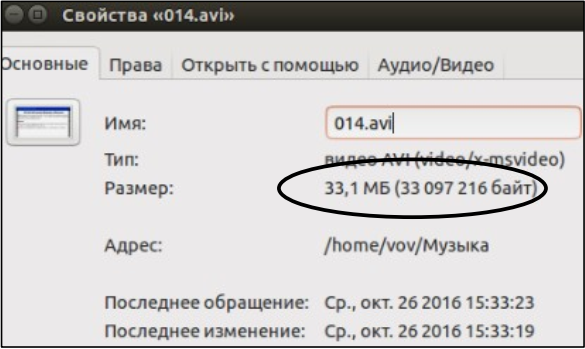
\includegraphics[scale=0.4]{ubuntu}
	\end{center}
	\column{5cm}
	\begin{center}
		Microsoft Windows 7\\
		\vskip 0.2cm
		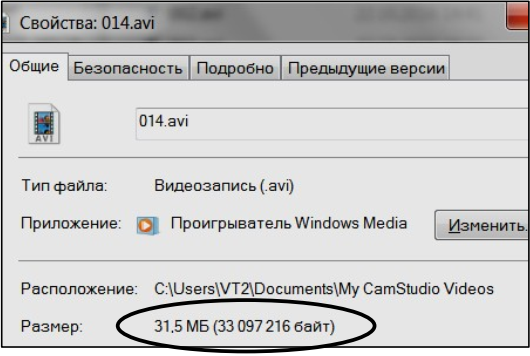
\includegraphics[scale=0.4]{windows}
	\end{center}
\end{columns}
\begin{center}
	33 097 216 байт --- это \color[rgb]{0,0.7,0.4}\textbf{33,1}\color{black} МБ или \color[rgb]{0,0.7,0.4} \textbf{31,5} \color{black} МБ?
\end{center}
\end{frame}